\documentclass[]{article}
\usepackage{lmodern}
\usepackage{amssymb,amsmath}
\usepackage{ifxetex,ifluatex}
\usepackage{fixltx2e} % provides \textsubscript
\ifnum 0\ifxetex 1\fi\ifluatex 1\fi=0 % if pdftex
  \usepackage[T1]{fontenc}
  \usepackage[utf8]{inputenc}
\else % if luatex or xelatex
  \ifxetex
    \usepackage{mathspec}
  \else
    \usepackage{fontspec}
  \fi
  \defaultfontfeatures{Ligatures=TeX,Scale=MatchLowercase}
\fi
% use upquote if available, for straight quotes in verbatim environments
\IfFileExists{upquote.sty}{\usepackage{upquote}}{}
% use microtype if available
\IfFileExists{microtype.sty}{%
\usepackage{microtype}
\UseMicrotypeSet[protrusion]{basicmath} % disable protrusion for tt fonts
}{}
\usepackage[margin=1in]{geometry}
\usepackage{hyperref}
\hypersetup{unicode=true,
            pdftitle={CoronaNet: A Dyadic Dataset of Government Responses to the COVID-19 Pandemic},
            pdfauthor={Cindy Cheng1,; Joan Barceló2; Allison Spencer Hartnett3; Robert Kubinec2; Luca Messerschmidt1},
            pdfborder={0 0 0},
            breaklinks=true}
\urlstyle{same}  % don't use monospace font for urls
\usepackage{longtable,booktabs}
\usepackage{graphicx,grffile}
\makeatletter
\def\maxwidth{\ifdim\Gin@nat@width>\linewidth\linewidth\else\Gin@nat@width\fi}
\def\maxheight{\ifdim\Gin@nat@height>\textheight\textheight\else\Gin@nat@height\fi}
\makeatother
% Scale images if necessary, so that they will not overflow the page
% margins by default, and it is still possible to overwrite the defaults
% using explicit options in \includegraphics[width, height, ...]{}
\setkeys{Gin}{width=\maxwidth,height=\maxheight,keepaspectratio}
\IfFileExists{parskip.sty}{%
\usepackage{parskip}
}{% else
\setlength{\parindent}{0pt}
\setlength{\parskip}{6pt plus 2pt minus 1pt}
}
\setlength{\emergencystretch}{3em}  % prevent overfull lines
\providecommand{\tightlist}{%
  \setlength{\itemsep}{0pt}\setlength{\parskip}{0pt}}
\setcounter{secnumdepth}{5}
% Redefines (sub)paragraphs to behave more like sections
\ifx\paragraph\undefined\else
\let\oldparagraph\paragraph
\renewcommand{\paragraph}[1]{\oldparagraph{#1}\mbox{}}
\fi
\ifx\subparagraph\undefined\else
\let\oldsubparagraph\subparagraph
\renewcommand{\subparagraph}[1]{\oldsubparagraph{#1}\mbox{}}
\fi

%%% Use protect on footnotes to avoid problems with footnotes in titles
\let\rmarkdownfootnote\footnote%
\def\footnote{\protect\rmarkdownfootnote}

%%% Change title format to be more compact
\usepackage{titling}

% Create subtitle command for use in maketitle
\providecommand{\subtitle}[1]{
  \posttitle{
    \begin{center}\large#1\end{center}
    }
}

\setlength{\droptitle}{-2em}

  \title{CoronaNet: A Dyadic Dataset of Government Responses to the COVID-19 Pandemic}
    \pretitle{\vspace{\droptitle}\centering\huge}
  \posttitle{\par}
    \author{Cindy Cheng\textsuperscript{1,*} \\ Joan Barceló\textsuperscript{2} \\ Allison Spencer Hartnett\textsuperscript{3} \\ Robert Kubinec\textsuperscript{2} \\ Luca Messerschmidt\textsuperscript{1}}
    \preauthor{\centering\large\emph}
  \postauthor{\par}
      \predate{\centering\large\emph}
  \postdate{\par}
    \date{April 10th, 2020}

\usepackage{tikzit}
\input{basic_oval.tikzstyles}
\linespread{1.6}
\usepackage{booktabs}
\usepackage{longtable}
\usepackage{array}
\usepackage{multirow}
\usepackage{wrapfig}
\usepackage{float}
\usepackage{colortbl}
\usepackage{pdflscape}
\usepackage{tabu}
\usepackage{threeparttable}
\usepackage{threeparttablex}
\usepackage[normalem]{ulem}
\usepackage{makecell}
\usepackage{xcolor}

\begin{document}
\maketitle
\begin{abstract}
As the COVID-19 pandemic spreads around the world, governments have implemented a broad set of policies to limit the spread of the pandemic. In this paper we present an initial release of a large hand-coded dataset of more than 4,500 separate policy announcements from governments around the world. This data is being made publicly available, in combination with other data that we have collected (including COVID-19 tests, cases, and deaths) as well as a number of country-level covariates. Due to the speed of the COVID-19 outbreak, we will be releasing this data on a daily basis with a 5-day lag for record validity checking. In a truly global effort, our team is comprised of more than 190 research assistants across 18 time zones and makes use of cloud-based managerial and data collection technology in addition to machine learning coding of news sources. We analyze the dataset with a Bayesian time-varying ideal point model showing the quick acceleration of more harsh policies across countries beginning in mid-March and continuing to the present. While some relatively low-cost policies like task forces and health monitoring began early, countries generally adopted more harsh measures within a narrow time window, suggesting strong policy diffusion effects.\footnote{We thank the very large number of research assistants who coded this data. Their names and affiliations are listed in the appendix. For the most current, up to date version of the dataset, please visit \url{http://coronanet-project.org} and also our Github page at \url{https://github.com/saudiwin/corona_tscs}. For more information on the exact variables collected, please see our publicly available codebook \href{https://docs.google.com/document/d/1zvNMpwj0onFvUZ_gLl4RRjqS-clbHv3TIX6EOHofsME/edit?usp=sharing}{at this link}.}
\end{abstract}

\textsuperscript{1} Hochschule für Politik at the Technical University of Munich (TUM) and TUM School of Governance\\
\textsuperscript{2} New York University Abu Dhabi\\
\textsuperscript{3} Yale University

\textsuperscript{*} Correspondence: \href{mailto:cindy.cheng@hfp.tum.de}{Cindy Cheng \textless{}\href{mailto:cindy.cheng@hfp.tum.de}{\nolinkurl{cindy.cheng@hfp.tum.de}}\textgreater{}}

\hypertarget{introduction}{%
\section{Introduction}\label{introduction}}

Governments all around the world have implemented an astonishing variety of policies in reaction to the COVID-19 pandemic. Policy makers and researchers however, have to date lacked access to the quality, up-to-date data they need for conducting rigorous analyses of whether, how, or to what degree these fast changing policies have worked in brunting the health, political and economic effects of the coronavirus. To address this concern, we present in this paper the CoronaNet COVID-19 Government Response Database, which provides fine-grained, dyadic data on policy actions taken by governments across the world since the Chinese government reported the COVID-19 outbreak on December 31, 2019. The dataset presented here covers all policy actions for 193 of countries\footnote{Note, we will include additional countries in future versions of the dataset.} up until 2020-04-11, for a total of 6755 events.

With the help of a team of over 190 research assistants in 18 time zones, we are releasing the data on a daily basis with a five-day lag between data collection and release to provide validation. We have further implemented ongoing random evaluation of coding efforts to ensure the best possible quality given the considerable time constraints. We believe that this data will permit crucial inference on both the determinants of these policies and their effects on societies, economies and the disease's spread.

More specifically, the CoronaNet database collects data on government policy actions taken against the coronavirus across the following dimensions on a daily basis:

\begin{itemize}
\tightlist
\item
  The type of government policy implemented (e.g.~quarantine, closure of schools {[}16 total{]} )
\item
  The level of government initiating the action (e.g.~national, provincial )
\item
  The geographical target of the policy action, if applicable (e.g.~national, provincial, municipal)
\item
  The human or material target of the policy action, if applicable (e.g.~travelers, health staff)
\item
  The directionality of the policy action, if applicable (e.g.~inbound, outbound, both)
\item
  The mechanism of travel that the policy action targets, if applicable (e.g.~flights, trains)
\item
  The compliance with the policy action (e.g.~mandatory, voluntary)
\item
  The timing of the policy action (e.g.~date announced, date implemented)
\end{itemize}

Data on government reactions the COVID-19 pandemic can not only help us understand which policies are more effective in addressing the spread and health outcomes of COVID-19, it can also forward our knowledge of, inter alia, the relative responsiveness of different political regime types (Przeworski, Stokes, and Manin 1999), the politics of crisis management (Boin et al. 2016), the development of financial crises (Kindleberger and Aliber 2011) and, the sociology of natural disasters (Tierney 2007). Moreover, given the exogenous timing of the initial COVID-19 outbreak in China, government policies made in reaction to the COVID-19 pandemic constitute the single largest natural experiment in recent memory, allowing researchers to improve causal inference in any number of fields. Indeed, how governments react to the COVID-19 epidemic will have long-lasting implications on a wide-range of social phenomena, from political institutions, (Pierson 2000) economic development (Nunn 2009) to environmental outcomes (Dasgupta et al. 2002). While scholars have always sought to understand how large-scale historical events have shaped contemporary phenomena, modern technological tools allow us to document such events more quickly and more precisely than ever before.

In what follows, we provide a description of the data, as well the application of our data in modeling the level of government policy activity over time. Using a Bayesian dynamic item-response theory model, we produce a statistically valid index that ranks countries in terms of their response to the pandemic, and also shows how quickly policy responses have changed over time. We document clear evidence of rapid policy diffusion of harsh measures opposing the virus, indicating some of the most extensive evidence of this type of diffusion ever documented. We then outline the methodology we used to collect the data.

\hypertarget{dataset-overview}{%
\section{Dataset Overview}\label{dataset-overview}}

Here we present some descriptive statistics to illustrate the type of data that the CoronaNet project is able to provide. First, however, we clarify the unit of analysis for each documented policies. Of the 6755 events in the dataset, we have identified 5750 unique events. That is, some events in the database are updates or changes to existing policies. We link such events overtime using a unique ID (\texttt{record\_id}). An event counts as an update if it deals with a change in either the:

\begin{enumerate}
\def\labelenumi{\arabic{enumi}.}
\tightlist
\item
  Time duration or\footnote{E.g. A country lengthens its quarantine to 28 days from 14 days.}
\item
  Strength of an existing policy in terms of either:

  \begin{enumerate}
  \def\labelenumii{\alph{enumii}.}
  \tightlist
  \item
    the nature of the policy\footnote{E.g. People can no longer leave their houses to go to work whereas before they could}
  \item
    compliance rules for the policy\footnote{E.g The quarantine used to be voluntary but now its mandatory}
  \item
    who the policy applies towards\footnote{E.g. The quarantine used to apply to people of all ages and now it only applies to the elderly.}
  \end{enumerate}
\end{enumerate}

A policy counts as a new entry and not an update if it deals with a change in any other dimension, e.g.~policy type, targeted country.

1 This variable documents the policy action initiated. It can take on only one of the following values:
2 Declaraction of Emergency
3 Quarantine
4 External Border Restrictions
5 Internal Border Restrictions
6 Restrictions of Mass Gatherings
7 Closure of Schools
8 Restriction of Non-Essential Government Services
9 Restriction of Non-Essential Businesses
10 Health Monitoring
11 Health Testing
12 Health Resource
13 Public Awareness Campaigns
14 New Task Force or Bureau

1 This variable documents the country from which a policy initiates, where applicable, and can take on only one of the following values:
2 National
3 Provincial/State
4 Municipality/City
5 Other governmental unit
6
7
8
9
10
11
12
13
14

1 This variable documents the geographical target of the policy. It can take on of the following variables (The exact geographical targets are also documented in other variables in the dataset):
2 All countries
3 One or more countries and one or more regional groupings
4 One or more countries, but not all countries
5 One or more regional groupings
6 A geographical or administrative unit within a country
7
8
9
10
11
12
13
14

1 This variable documents the human or material targets of a policy, where applicable, and can take on only one of the following values:
2 All (Travelers + Residents)
3 All Travelers (Citizen Travelers + Foreign Travelers)
4 Citizen Travelers
5 Foreign Travelers
6 All Residents (Citizen Residents + Foreign Residents)
7 Citizen Residents
8 Foreign Residents
9 All Foreign Nationals
10 All Citizens
11 Health Staff
12 Health-related Supplies
13
14

1 This variable documents the direction of travel a policy targets, where applicable, and can take on only one of the following values:
2 Inbound
3 Outbound
4 Inbound/Outbound
5
6
7
8
9
10
11
12
13
14

1 This variable documents the mode of travel a policy targets, where applicable, and can take on one or more of the following values:
2 All Mechansims (except visa restrictions)
3 Flights
4 Land Border
5 Trains
6 Buses
7 Seaports
8 Ferries
9 Cruises
10 Visas
11
12
13
14

1 This variable documents degree to which a policy must be complied with and can take on one or more of the following values:
2 Mandatory with Legal Penalties
3 Mandatory with Fines
4 Mandatory with Excpetions
5 Recommended/Voluntary
6
7
8
9
10
11
12
13
14

1 This variable documents the entity enforcing a policy and can take on one or more of the following values:
2 National Government
3 Ministry/Department of Health
4 Military
5 Provincial/State Government
6 Municipal/City Government
7 Police
8 Other
9
10
11
12
13
14

1 The following are separate variables in the dataset which document when a policy is announced, starts and ends repsectively:
2 Date Announced
3 Date Starts
4 Date Ends
5
6
7
8
9
10
11
12
13
14

Table \ref{tab:desctab} shows the number of records for each policy type, the number of unique countries for each policy type, and also how many countries are targeted in total by each policy type.\footnote{Future versions of the dataset will also include more detailed information for some policy categories. For example, among other things, we are also collecting information on the types of `health resources' (e.g.~masks, hospitals, doctors ) and types of `restrictions of non-essential business activities' (e.g.~retail businesses, restaurants/bars). Where applicable, we are also collecting information on the volume of a certain policy (e.g.~the number of masks, hospitals and doctors.). We will also be including a variable which documents which institution is responsible for enforcing a certain policy (e.g.~national government, military).} We note that these are cumulative totals for these different categories in the data.

\begin{table}[!h]

\caption{\label{tab:desctab}Descriptive Information about the CoronaNet Government Response Dataset}
\centering
\begin{tabular}{>{\raggedright\arraybackslash}p{4cm}>{\raggedleft\arraybackslash}p{2.5cm}>{\raggedleft\arraybackslash}p{2.5cm}>{\raggedleft\arraybackslash}p{2.5cm}>{\raggedleft\arraybackslash}p{2.5cm}}
\toprule
Type & Total Number of Policies & Number of Countries & Number of Targeted Countries & \% With Mandatory Enforcement\\
\midrule
\rowcolor{gray!6}  Closure of Schools & 1248 & 157 & 3 & 86\\
Curfew & 175 & 87 & 21 & 97\\
\rowcolor{gray!6}  Declaration of Emergency & 318 & 109 & 1 & 82\\
External Border Restrictions & 4061 & 178 & 201 & 90\\
\rowcolor{gray!6}  Health Monitoring & 607 & 99 & 198 & 75\\
\addlinespace
Health Resources & 1331 & 128 & 125 & 54\\
\rowcolor{gray!6}  Health Testing & 249 & 76 & 100 & 78\\
Internal Border Restrictions & 253 & 104 & 94 & 87\\
\rowcolor{gray!6}  New Task Force or Bureau & 217 & 90 & 1 & 49\\
Other Policy Not Listed Above & 555 & 119 & 1 & 61\\
\addlinespace
\rowcolor{gray!6}  Public Awareness Campaigns & 392 & 115 & 1 & 24\\
Quarantine/Lockdown & 2828 & 145 & 202 & 80\\
\rowcolor{gray!6}  Restriction of Non-Essential Businesses & 1240 & 125 & 1 & 92\\
Restriction of Non-Essential Government Services & 206 & 84 & 1 & 83\\
\rowcolor{gray!6}  Restrictions of Mass Gatherings & 521 & 148 & 2 & 86\\
\addlinespace
Social Distancing & 382 & 113 & 2 & 72\\
\bottomrule
\end{tabular}
\end{table}

In addition, we can look at the cumulative incidence of different types of policies in our data over time, as we show in Figure \ref{fig:overtime}. The figure shows that relatively easy to implement policies like the forming of task forces, public awareness campaigns, and efforts to increase health resources came relatively early. More restrictive policies like curfews, closures of schools and mass gatherings arrived later in the course of the pandemic.

\begin{figure}
\centering
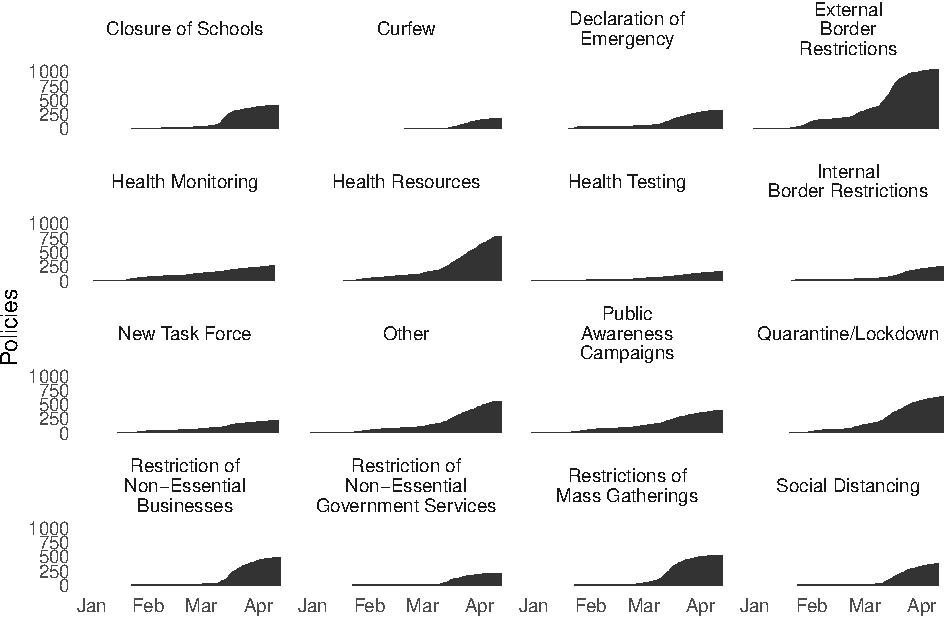
\includegraphics{corona_wp_files/figure-latex/overtime-1.pdf}
\caption{\label{fig:overtime}Cumulative Incidence of Policy Event Types Over Time}
\end{figure}

We can also explore the extent to which other countries are affected by policies that can have a geographic target outside the policy initiator (e.g.~`external border restrictions', `quarantine'). For example, in Figure @ref(fig:biofabric\_europe), we map a network of bans on inbound flights to European countries initiated by European countries\footnote{In this paper, the following countries are defined as being in Europe: Albania, Andorra, Armenia, Austria, Belarus, Belgium, Bosnia and Herzegovina, Bulgaria, Croatia, Cyprus, Czech Republic, Denmark, Estonia, Finland, France, Georgia, Germany, Greece, Hungary, Iceland, Ireland, Italy, Kosovo, Latvia, Liechtenstein, Lithuania, Luxembourg, Macedonia, Malta, Moldova, Monaco, Montenegro, Netherlands, Norway, Poland, Portugal, Romania, San Marino, Serbia, Slovakia, Slovenia, Spain, Sweden, Switzerland, Ukraine, United Kingdom, and the Vatican} as of March 15, 2020. In the plot, each horizontal line represents a potential geographical target of a flight ban. The vertical lines denote whether there was such a flight ban and the arrow of the vertical line indicates the direction in which the ban is applied.\footnote{(See Longabaugh 2012 for more information on how to interpret this plot.)} For instance, the figure shows that by March 15, 2020, the governments of Poland and San Marino had banned all flights into Poland and San Marino respectively while the government of the autonomous region of Madeira, Portugal had banned flights from Denmark, Finland, France, Germany, Spain, and Switzerland.


\includegraphics{corona_wp_files/figure-latex/biofabric_europe-1.pdf}

\hypertarget{government-response-severity-index}{%
\section{Government Response Severity Index}\label{government-response-severity-index}}

In this section we briefly present our new index for tracking the relative intensity of government policies targeting COVID-19 across countries and over time. The model is a version of item-response theory that incorporates over-time trends (Kubinec 2019), permitting inference on how a latent construct, in this case policy stringency, is responding to changes in the pandemic. To fit the model, the different policy types shown in Table \ref{tab:desctab} were coded dichotomously, with a value of 1 if enforcement of the policy was mandatory, and 0 otherwise. As a result, the model estimates whether mandatory policies for each category exist for each country on each day. The country-level stringency score is allowed to vary over time in a random-walk process with a country-specific variance parameter (i.e., to incorporate heteroskedasticity).

The advantage of employing a statistical model, rather than simply summing across policies, is that the index ends up as a weighted average, where the weights are derived from the probability that a certain policy is enforced. In other words, while many countries set up task forces, relatively few imposed curfews at an early stage. As a result, the model adjusts for these distinctions, producing a score that aggregates across the patterns in the data. Because over-time trends are explicitly included and jointly estimated with the latent parameters, the model will implicitly up-weight countries that took harsher measures earlier.

Furthermore, because the model is stochastic, it is robust to coding errors of the kind that often occur in these types of datasets. As we discuss in our validation section, while we are continuing to validate the data on a daily basis, the massive speed and scope of data collection means that we cannot identify all issues with the data in real time. However, the measurement model employed only requires us to assume that on average the policy codings are correct, not that they are correct for each instance. Coding error, such as incorrectly selecting a policy type, will propagate through the model as higher uncertainty intervals, but will not affect average posterior estimates. As our data quality improves, and we are able to collect more data over time, the model will produce more variegated estimates with smaller uncertainty intervals.

Figure \ref{fig:plotindex} shows the estimated index scores for the 0 countries in our dataset at present. Of course, a caveat with the index is that we may be missing some possible policy measures that have occurred due to the difficulty in finding them in published sources. However, there is still clear differentiation within the index in terms of when policies were imposed, with some countries starting to impose policies much earlier than others. Furthermore, there is a clear break about March 1st when countries began to impose more stringent policies across the world.

Figure \ref{fig:plotindex} shows the estimated index scores for the 0 countries in our dataset at present. Of course, a caveat with the index is that we may be missing some possible policy measures that have occurred due to the difficulty in finding them in published sources. However, there is still clear differentiation within the index in terms of when policies were imposed, with some countries starting to impose policies much earlier than others. Furthermore, there is a clear break about March 1st when countries began to impose more stringent policies across the world.

\begin{figure}
\centering
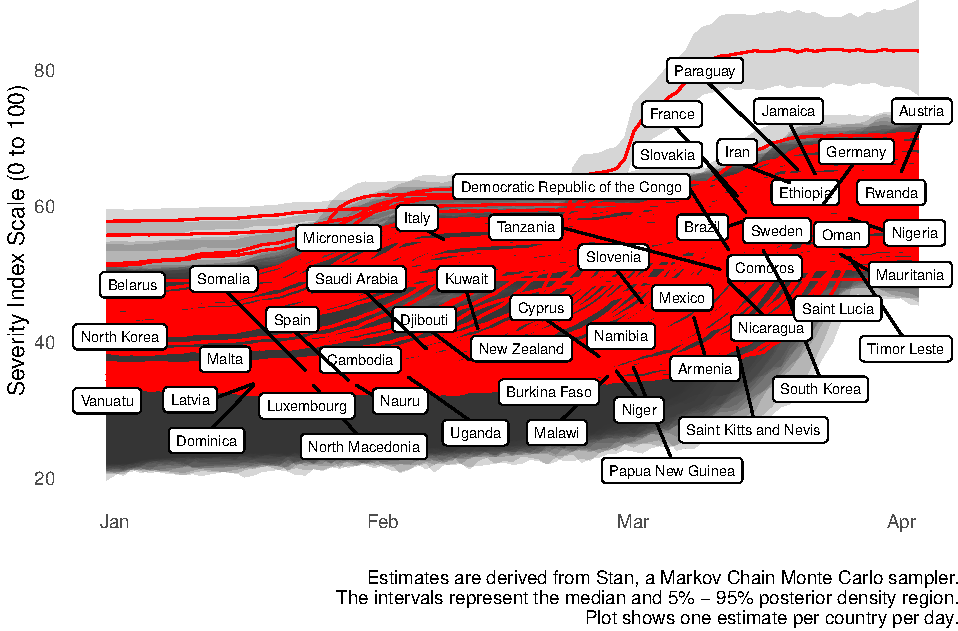
\includegraphics{corona_wp_files/figure-latex/plotindex-1.pdf}
\caption{\label{fig:plotindex}CoronaNet Time-Varying Index of National Policy Activity of Measures Opposing COVID-19 Pandemic}
\end{figure}

Table \ref{tab:rankcount} shows the rank of countries for the index at present. An important note about these results is that the rank only measures the posterior median, or most likely estimate, but the 5\% - 95\% uncertainty interval shows that substantial uncertainty exists in comparing neighboring countries in the index. More certain comparisons can be made between the top, middle and bottom third of countries, while within these categories the estimates are not precise enough to make finer-grained distinctions with confidence.

With this caveat in mind, San Marino occupies the highest position, likely because of harsh lockdowns imposed as a result of the outbreak in northern Italy that occurred relatively early. Slovenia has had a nationwide lockdown in place for several weeks, while Azerbaijan took early action to close its borders with Iran in February after the outbreak started. It is important to note the uncertainty in the index measures, as the top 10 countries cannot be distinguished from each other in severity except for San Marino. We believe these uncertainty intervals are important to capture the difficulty in using published policies to compare countries. However, we also see substantial value in this index, particularly in its ability to show change over time.

\begin{longtable}{>{\raggedright\arraybackslash}p{4cm}>{\raggedleft\arraybackslash}p{2.5cm}>{\raggedleft\arraybackslash}p{2.5cm}>{\raggedleft\arraybackslash}p{2.5cm}>{\raggedleft\arraybackslash}p{2.5cm}}
\caption{\label{tab:rankcount}Rank of Countries by National Policy Activity Index as of April 3rd, 2020}\\
\toprule
Country & Rank & 5\% Low Score & Median Score & 95\% High Score\\
\midrule
\rowcolor{gray!6}  Gabon & 1 & 61.3 & 63.6 & 66.4\\
Croatia & 2 & 59.3 & 62.8 & 66.1\\
\rowcolor{gray!6}  United Arab Emirates & 3 & 58.6 & 62.4 & 66.9\\
Guatemala & 4 & 58.8 & 61.8 & 65.0\\
\rowcolor{gray!6}  Slovenia & 5 & 58.2 & 61.5 & 64.7\\
\addlinespace
San Marino & 6 & 57.2 & 61.5 & 66.0\\
\rowcolor{gray!6}  Eswatini & 7 & 57.1 & 61.3 & 65.6\\
Antigua and Barbuda & 8 & 58.0 & 61.2 & 64.1\\
\rowcolor{gray!6}  Hungary & 9 & 58.2 & 61.2 & 65.2\\
Poland & 10 & 56.5 & 61.1 & 66.3\\
\addlinespace
\rowcolor{gray!6}  Latvia & 11 & 59.5 & 61.1 & 62.8\\
Grenada & 12 & 55.8 & 61.1 & 66.4\\
\rowcolor{gray!6}  Iraq & 13 & 58.4 & 60.9 & 63.6\\
Mali & 14 & 59.2 & 60.9 & 63.1\\
\rowcolor{gray!6}  Albania & 15 & 57.8 & 60.7 & 63.8\\
\addlinespace
Romania & 16 & 58.0 & 60.7 & 63.4\\
\rowcolor{gray!6}  Israel & 17 & 58.8 & 60.7 & 62.5\\
Saudi Arabia & 18 & 57.3 & 60.7 & 64.1\\
\rowcolor{gray!6}  Peru & 19 & 59.2 & 60.6 & 62.3\\
Democratic Republic of the Congo & 20 & 58.2 & 60.6 & 63.0\\
\addlinespace
\rowcolor{gray!6}  Costa Rica & 21 & 59.8 & 60.6 & 61.7\\
Botswana & 22 & 57.0 & 60.5 & 64.4\\
\rowcolor{gray!6}  Bulgaria & 23 & 58.3 & 60.5 & 62.6\\
Saint Kitts and Nevis & 24 & 57.9 & 60.5 & 62.8\\
\rowcolor{gray!6}  Netherlands & 25 & 55.5 & 60.5 & 65.8\\
\addlinespace
Madagascar & 26 & 57.6 & 60.4 & 63.0\\
\rowcolor{gray!6}  Austria & 27 & 60.0 & 60.3 & 60.9\\
Belgium & 28 & 58.5 & 60.2 & 62.7\\
\rowcolor{gray!6}  Russia & 29 & 58.5 & 60.2 & 62.0\\
Kuwait & 30 & 59.7 & 60.2 & 61.0\\
\addlinespace
\rowcolor{gray!6}  Switzerland & 31 & 57.4 & 60.1 & 62.4\\
Ukraine & 32 & 56.9 & 60.1 & 63.6\\
\rowcolor{gray!6}  Malta & 33 & 53.3 & 60.1 & 67.0\\
Lesotho & 34 & 56.2 & 60.1 & 63.7\\
\rowcolor{gray!6}  Cyprus & 35 & 58.7 & 60.1 & 61.5\\
\addlinespace
Uruguay & 36 & 51.8 & 60.0 & 67.6\\
\rowcolor{gray!6}  Angola & 37 & 57.2 & 60.0 & 62.7\\
Djibouti & 38 & 51.3 & 60.0 & 71.0\\
\rowcolor{gray!6}  Monaco & 39 & 57.6 & 60.0 & 62.6\\
Luxembourg & 40 & 55.0 & 59.9 & 64.9\\
\addlinespace
\rowcolor{gray!6}  Finland & 41 & 58.9 & 59.9 & 61.0\\
Spain & 42 & 58.6 & 59.9 & 61.0\\
\rowcolor{gray!6}  Uganda & 43 & 56.5 & 59.9 & 63.6\\
Italy & 44 & 57.6 & 59.9 & 62.3\\
\rowcolor{gray!6}  Eritrea & 45 & 56.4 & 59.9 & 63.3\\
\addlinespace
Chile & 46 & 56.7 & 59.8 & 63.0\\
\rowcolor{gray!6}  Colombia & 47 & 59.0 & 59.8 & 60.5\\
Kenya & 48 & 58.9 & 59.7 & 60.6\\
\rowcolor{gray!6}  Jordan & 49 & 47.1 & 59.7 & 70.8\\
Denmark & 50 & 53.2 & 59.7 & 66.5\\
\addlinespace
\rowcolor{gray!6}  Ireland & 51 & 58.2 & 59.7 & 61.1\\
North Macedonia & 52 & 59.3 & 59.7 & 60.1\\
\rowcolor{gray!6}  United Kingdom & 53 & 55.5 & 59.7 & 64.3\\
Kazakhstan & 54 & 57.5 & 59.7 & 61.9\\
\rowcolor{gray!6}  Gambia & 55 & 59.1 & 59.7 & 60.4\\
\addlinespace
Azerbaijan & 56 & 59.5 & 59.7 & 59.9\\
\rowcolor{gray!6}  Morocco & 57 & 57.7 & 59.7 & 61.7\\
Moldova & 58 & 55.4 & 59.6 & 63.3\\
\rowcolor{gray!6}  Qatar & 59 & 57.2 & 59.6 & 62.4\\
South Africa & 60 & 58.6 & 59.6 & 60.7\\
\addlinespace
\rowcolor{gray!6}  Jamaica & 61 & 58.8 & 59.6 & 60.4\\
Mauritania & 62 & 56.7 & 59.6 & 63.0\\
\rowcolor{gray!6}  Hong Kong & 63 & 59.0 & 59.6 & 60.1\\
Lithuania & 64 & 58.9 & 59.6 & 60.4\\
\rowcolor{gray!6}  Tonga & 65 & 53.7 & 59.5 & 64.9\\
\addlinespace
Germany & 66 & 53.9 & 59.5 & 65.1\\
\rowcolor{gray!6}  Samoa & 67 & 59.1 & 59.5 & 60.0\\
Ivory Coast & 68 & 57.2 & 59.5 & 61.8\\
\rowcolor{gray!6}  Portugal & 69 & 59.2 & 59.5 & 59.8\\
Ethiopia & 70 & 57.7 & 59.5 & 60.9\\
\addlinespace
\rowcolor{gray!6}  Niger & 71 & 56.8 & 59.5 & 61.9\\
Slovakia & 72 & 56.8 & 59.5 & 62.4\\
\rowcolor{gray!6}  China & 73 & 58.1 & 59.5 & 60.9\\
Liechtenstein & 74 & 57.6 & 59.5 & 61.6\\
\rowcolor{gray!6}  Ecuador & 75 & 57.1 & 59.5 & 61.9\\
\addlinespace
Cameroon & 76 & 55.3 & 59.4 & 63.2\\
\rowcolor{gray!6}  Kyrgyzstan & 77 & 58.1 & 59.4 & 60.7\\
Dominica & 78 & 58.3 & 59.4 & 60.8\\
\rowcolor{gray!6}  El Salvador & 79 & 56.9 & 59.4 & 62.1\\
Cambodia & 80 & 57.8 & 59.4 & 61.0\\
\addlinespace
\rowcolor{gray!6}  Bolivia & 81 & 52.9 & 59.4 & 65.2\\
Mexico & 82 & 57.6 & 59.4 & 61.0\\
\rowcolor{gray!6}  Sudan & 83 & 55.8 & 59.4 & 62.9\\
Turkey & 84 & 57.8 & 59.3 & 61.2\\
\rowcolor{gray!6}  Somalia & 85 & 56.3 & 59.3 & 62.5\\
\addlinespace
Togo & 86 & 57.7 & 59.3 & 61.1\\
\rowcolor{gray!6}  Honduras & 87 & 59.0 & 59.3 & 59.6\\
Iran & 88 & 59.0 & 59.3 & 59.7\\
\rowcolor{gray!6}  Mongolia & 89 & 58.6 & 59.3 & 60.0\\
Serbia & 90 & 52.6 & 59.3 & 66.3\\
\addlinespace
\rowcolor{gray!6}  Paraguay & 91 & 58.5 & 59.3 & 59.9\\
Australia & 92 & 53.6 & 59.3 & 64.9\\
\rowcolor{gray!6}  Burkina Faso & 93 & 58.4 & 59.3 & 60.1\\
Tanzania & 94 & 58.4 & 59.3 & 60.2\\
\rowcolor{gray!6}  Egypt & 95 & 58.9 & 59.3 & 59.6\\
\addlinespace
Bhutan & 96 & 57.6 & 59.2 & 60.9\\
\rowcolor{gray!6}  Palestine & 97 & 58.2 & 59.2 & 60.2\\
France & 98 & 57.6 & 59.2 & 60.9\\
\rowcolor{gray!6}  Pakistan & 99 & 58.7 & 59.2 & 59.7\\
Benin & 100 & 55.4 & 59.2 & 62.8\\
\addlinespace
\rowcolor{gray!6}  Brazil & 101 & 48.5 & 59.2 & 71.0\\
Papua New Guinea & 102 & 57.4 & 59.2 & 61.1\\
\rowcolor{gray!6}  Algeria & 103 & 57.5 & 59.2 & 61.0\\
Mozambique & 104 & 58.9 & 59.2 & 59.5\\
\rowcolor{gray!6}  Philippines & 105 & 51.4 & 59.2 & 67.5\\
\addlinespace
Senegal & 106 & 56.6 & 59.2 & 62.4\\
\rowcolor{gray!6}  Estonia & 107 & 55.2 & 59.2 & 63.9\\
Oman & 108 & 58.7 & 59.2 & 59.6\\
\rowcolor{gray!6}  Cuba & 109 & 56.6 & 59.2 & 61.7\\
Suriname & 110 & 58.7 & 59.2 & 59.7\\
\addlinespace
\rowcolor{gray!6}  Tunisia & 111 & 57.5 & 59.2 & 61.0\\
Argentina & 112 & 57.2 & 59.1 & 61.1\\
\rowcolor{gray!6}  Taiwan & 113 & 58.6 & 59.1 & 59.7\\
Sierra Leone & 114 & 55.5 & 59.1 & 62.5\\
\rowcolor{gray!6}  Thailand & 115 & 55.8 & 59.1 & 62.3\\
\addlinespace
Equatorial Guinea & 116 & 56.6 & 59.1 & 61.9\\
\rowcolor{gray!6}  Rwanda & 117 & 56.1 & 59.1 & 62.9\\
Kiribati & 118 & 51.6 & 59.1 & 66.7\\
\rowcolor{gray!6}  Trinidad and Tobago & 119 & 56.4 & 59.1 & 61.8\\
Guyana & 120 & 55.9 & 59.1 & 62.7\\
\addlinespace
\rowcolor{gray!6}  Vanuatu & 121 & 58.2 & 59.1 & 59.9\\
Namibia & 122 & 53.8 & 59.1 & 64.8\\
\rowcolor{gray!6}  Solomon Islands & 123 & 56.9 & 59.1 & 62.1\\
Republic of the Congo & 124 & 57.5 & 59.0 & 60.6\\
\rowcolor{gray!6}  Saint Vincent and the Grenadines & 125 & 57.9 & 59.0 & 60.4\\
\addlinespace
Sao Tome and Principe & 126 & 56.9 & 59.0 & 61.2\\
\rowcolor{gray!6}  Brunei & 127 & 54.5 & 59.0 & 63.7\\
Bahamas & 128 & 53.6 & 59.0 & 64.4\\
\rowcolor{gray!6}  South Sudan & 129 & 53.9 & 59.0 & 64.1\\
Zambia & 130 & 53.8 & 59.0 & 64.9\\
\addlinespace
\rowcolor{gray!6}  Iceland & 131 & 58.5 & 59.0 & 59.4\\
Panama & 132 & 58.0 & 59.0 & 60.0\\
\rowcolor{gray!6}  Sri Lanka & 133 & 55.0 & 58.8 & 62.7\\
Sweden & 134 & 55.9 & 58.8 & 61.2\\
\rowcolor{gray!6}  Belarus & 135 & 57.7 & 58.8 & 60.1\\
\addlinespace
Burundi & 136 & 54.3 & 58.8 & 62.6\\
\rowcolor{gray!6}  Myanmar & 137 & 58.0 & 58.7 & 59.5\\
Central African Republic & 138 & 56.3 & 58.6 & 61.7\\
\rowcolor{gray!6}  Guinea & 139 & 54.5 & 58.5 & 61.9\\
Uzbekistan & 140 & 53.2 & 58.5 & 64.6\\
\addlinespace
\rowcolor{gray!6}  Barbados & 141 & 57.3 & 58.5 & 59.7\\
Malawi & 142 & 52.5 & 58.4 & 63.3\\
\rowcolor{gray!6}  Indonesia & 143 & 57.5 & 58.3 & 59.0\\
Turkmenistan & 144 & 54.6 & 58.3 & 62.9\\
\rowcolor{gray!6}  Czechia & 145 & 57.6 & 58.2 & 59.0\\
\addlinespace
Ghana & 146 & 55.9 & 58.2 & 61.2\\
\rowcolor{gray!6}  Dominican Republic & 147 & 56.7 & 58.1 & 60.1\\
Japan & 148 & 57.5 & 58.1 & 58.7\\
\rowcolor{gray!6}  Georgia & 149 & 54.5 & 58.1 & 61.6\\
Timor Leste & 150 & 54.7 & 58.1 & 61.7\\
\addlinespace
\rowcolor{gray!6}  Lebanon & 151 & 56.1 & 58.0 & 60.5\\
Fiji & 152 & 54.8 & 57.9 & 61.4\\
\rowcolor{gray!6}  Vietnam & 153 & 54.2 & 57.8 & 61.0\\
Nepal & 154 & 56.8 & 57.7 & 58.5\\
\rowcolor{gray!6}  Libya & 155 & 54.0 & 57.7 & 63.5\\
\addlinespace
Singapore & 156 & 52.8 & 57.6 & 62.0\\
\rowcolor{gray!6}  Norway & 157 & 54.9 & 57.6 & 60.3\\
Canada & 158 & 52.9 & 57.6 & 63.4\\
\rowcolor{gray!6}  Maldives & 159 & 52.1 & 57.6 & 62.6\\
Tajikistan & 160 & 50.4 & 57.5 & 63.5\\
\addlinespace
\rowcolor{gray!6}  Zimbabwe & 161 & 52.8 & 57.5 & 61.8\\
Venezuela & 162 & 52.9 & 57.5 & 61.7\\
\rowcolor{gray!6}  Nigeria & 163 & 54.3 & 57.5 & 60.4\\
Montenegro & 164 & 53.4 & 57.4 & 60.5\\
\rowcolor{gray!6}  Andorra & 165 & 54.6 & 57.4 & 60.1\\
\addlinespace
New Zealand & 166 & 50.3 & 57.3 & 63.3\\
\rowcolor{gray!6}  United States & 167 & 56.3 & 57.3 & 58.1\\
Afghanistan & 168 & 54.0 & 57.3 & 61.2\\
\rowcolor{gray!6}  Comoros & 169 & 51.8 & 57.3 & 62.6\\
Syria & 170 & 53.3 & 57.3 & 60.4\\
\addlinespace
\rowcolor{gray!6}  Bangladesh & 171 & 55.1 & 57.0 & 59.4\\
South Korea & 172 & 51.8 & 56.5 & 60.4\\
\rowcolor{gray!6}  Seychelles & 173 & 52.4 & 56.4 & 63.1\\
Bosnia and Herzegovina & 174 & 48.1 & 56.3 & 61.9\\
\rowcolor{gray!6}  Micronesia & 175 & 45.5 & 56.3 & 67.6\\
\addlinespace
Nauru & 176 & 49.8 & 56.3 & 61.3\\
\rowcolor{gray!6}  Liberia & 177 & 48.4 & 56.1 & 61.4\\
North Korea & 178 & 48.5 & 56.0 & 62.4\\
\rowcolor{gray!6}  Tuvalu & 179 & 48.4 & 55.9 & 61.5\\
Armenia & 180 & 50.7 & 55.8 & 59.9\\
\addlinespace
\rowcolor{gray!6}  Cabo Verde & 182 & 48.3 & 55.3 & 60.0\\
India & 183 & 45.0 & 54.0 & 59.5\\
\rowcolor{gray!6}  Macau & 184 & 40.8 & 52.3 & 58.4\\
Saint Lucia & 185 & 36.6 & 51.1 & 59.4\\
\rowcolor{gray!6}  Yemen & 186 & 34.3 & 48.9 & 56.4\\
\bottomrule
\end{longtable}

Finally, we note in Figure \ref{fig:plotindex} the strong evidence of policy diffusion effects. While information about COVID-19 existed at least as early as January, we do not see large-scale changes occurring in severity scores until March. Furthermore, the trajectories are highly non-linear, with a large number of countries quickly transitioning from relatively low to relatively high scores. This tandem movement is a strong indication of policy diffusion as countries adopted similar policies across time and space as opposed to a more linear learning process.

\hypertarget{methodology}{%
\section{Methodology}\label{methodology}}

To collect the data, we recruited more than 190 research assistants (RAs) from colleges and universities around the world, representing 18 out of the 24 time zones.\footnote{For more information on the individual RAs, please visit \url{http://coronanet-project.org/}} Data collection started on March 28, 2020 and has proceeded very rapidly, reaching 6755 records as of the date of this article. Each RA is responsible for tracking government policy actions for at least one country. RAs were allocated depending on their background, language skills and expressed interest in certain countries.\footnote{Note depending on the level of policy coordination at the national level, certain countries were assigned multiple RAs, e.g.~the United States, Germany, or France.}

We have also partnered with the machine learning company Jataware to automate the collection of more than 200,000 news articles from around the world related to COVID-19.\footnote{We thank Brandon Rose and Jataware for making the news database available to this project.} Jataware employs a natural language processing (NLP) classifier using Bidirectional Encoder Representations from Transformers (BERT) to detect whether a given article is indicative of a governmental policy intervention related to COVID-19. They then apply a secondary NLP classifier to categorize the type of policy intervention (e.g.~``state of emergency'', ``shelter-in-place'', ``quarantine'', ``travel restrictions'', etc). Next, Jataware extracts the geospatial and temporal extent of the policy intervention (e.g.~``Washington DC'' and ``March 15, 2020'') whenever possible. The resulting list of news sources is then provided to our RAs for manual coding and further data validation.

As researchers learn more about the various health, economic, and social effects of the coronavirus pandemic, it is crucial that they have access to data that is reliable, valid, and timely (to the greatest extent possible). We have adopted the following data collection methodology that we believe optimizes over all three of these constraints.

\hypertarget{data-collection-software-instrument}{%
\subsection{Data Collection Software Instrument}\label{data-collection-software-instrument}}

We designed a Qualtrics survey with survey questions about different aspects of a government policy action to streamline the CoronaNet data collection effort. With this tool, RAs can easily and efficiently document different policy actions by answering the relevant questions posed in the survey. For example, instead of entering the country that initiated a policy action into a spreadsheet, RAs answer the following question in the survey: ``From what country does this policy originate from?'' and choose from the available options given in the survey.

By using a survey instrument to collect data, we are able to systematize the collection of very fine-grained data while avoiding coding errors common to tools like shared spreadsheets. The value of this approach of course, depends on the comprehensiveness of the questions posed in the survey, especially in terms of the universe of policy actions that countries have implemented against COVID-19. For example, if the survey only allowed RAs to select `quarantines' as a government policy, it would not capture any data on `external border restrictions', which would seriously reduce the value of the resulting data.

As such, to ensure the comprehensiveness of the data, before designing the survey, we collected in depth, over-time data on policy actions taken by one country, Taiwan, since the beginning of the outbreak as well as cross-national data on travel bans implemented by most countries for a total of 245 events.\footnote{The specific data source the PI cross referenced for this effort was the March 20, 2020 version of the following New York Times article Salcedo, Andrea and Gina Cherelus, ``Coronavirus Travel Restrictions, Across the Globe'' \emph{New York Times}, 20 March 2020, \url{https://www.nytimes.com/article/coronavirus-travel-restrictions.html}} We chose to focus on Taiwan on because of its relative success, as of March 28, 2020, in limiting the negative health consequences of the coronavirus within its borders.\footnote{Beech, Hannah. ``Tracking the Coronavirus: How Crowded Asian Cities Tackled an Epidemic.'' \emph{New York Times} 18 March 2020 \url{https://www.nytimes.com/2020/03/17/world/asia/coronavirus-singapore-hong-kong-taiwan.html}} As such, it seems likely that other countries may choose to emulate some of the policy measures that Taiwan had implemented, which helps increase the comprehensiveness of the questions we ask in our survey. Meanwhile, by also investigating variation in how different countries around the world have implemented travel restrictions, we have also helped ensure that our survey is able to comprehensively document variation in how an important and commonly used policy tool is applied, e.g.~restrictions of different methods of travel (e.g.~flights, cruises), restrictions across borders and within borders, restrictions targeted toward people of different status (e.g.~citizens, travelers).

There are many additional benefits of using a survey instrument for data collection, especially in terms of ensuring the reliability and validity of the resulting the data:

\begin{enumerate}
\def\labelenumi{\arabic{enumi}.}
\item
  \emph{Preventing unforced measurement error.} RAs are prevented from entering data into incorrect fields or unknowingly overwriting existing data---as would be possible with manual data entry into a spreadsheet---because RAs can only document one policy action at a time in a given iteration of a survey and do not have access to the full spreadsheet when they are entering in the data.
\item
  \emph{Standardizing responses.} We are able to ensure that RAs can only choose among standardized responses to the survey questions, which increases the reliability of the data and also reduces the likelihood of measurement error. For example, when RAs choose different dates that we would like them to document (e.g., the date a policy was announced) they are forced to choose from a calendar embedded into the survey which systemizes the day, month and year format that the date is recorded in.
\item
  \emph{Minimizing measurement error.} A survey instrument allows coding different conditional logics for when certain survey questions are posed. This technique obviates the occurence of logical fallacies in our data. For example, we are able to avoid a situations where an RA might accidentally code the United States as having closed all schools in another country.
\item
  \emph{Reduction of missing data.} We are able to reduce the amount of missing data in the dataset by using the forced response option in Qualtrics. Where there is truly missing data due, there is a text entry at the end of the survey where RAs can describe what difficulties they encountered in collecting information for a particular policy event.
\item
  \emph{Reliability of the responses.} We increase the reliability of the documentation for each policy by embedding descriptions of different possible responses within the survey. For example, in the survey question where RAs are asked to identify the policy type (`type' variable, see Codebook), the survey question includes pop-up buttons which allow RAs to easily get descriptions and examples of each possible policy type. Such pop-up buttons were also made available for the survey questions which code for the people or materials a policy was targed at (`target\_who\_what') and whether the policy was inbound, outbound or both (`target\_direction'). Embedding such information in the dataset both clarifies the distinction between different answer choices and increases the efficiency of the policy documentation process (as RAs are not obliged to refer back and forth from the survey to the codebook).
\item
  \emph{Linking observations.} The use of a survey instrument allows us to easily link policy events together over time should there be updates to existing policies. Once coded, each policy is given a unique Record ID, which RAs can easily look up, reference and link to if they need to update a particular policy.
\end{enumerate}

\hypertarget{ra-training}{%
\subsection{RA Training}\label{ra-training}}

All RAs watch a mandatory 50 minute video training of the survey instrument which explains how to use the survey instrument. RAs are also provided with written guidelines on how to collect data and a comprehensive codebook. To briefly describe it here, the written guidelines provide a definition of what counts as a new or updated policy (see Data section for more details) and provides a checklist for RAs to follow in order to identify and document different policies. In the checklist, RAs are instructed to find policies by checking the sources in the order given in the guidelines to identify policies, to document the relevant information into the survey and to save and upload a document of the source they found for each policy into Qualtrics. The codebook meanwhile provides descriptions and examples of the different possible response options in the survey. Using a training video and the written codebook also has the added benefit of helping us efficiently disseminate the information RAs need to use the survey experiment consistently.

In order to participate as an RA in this project, RAs must fill out a form\footnote{See \href{https://docs.google.com/forms/d/e/1FAIpQLSeybAW0DC0UE1x2EqLiTifVFuSUxqJLGFB8VI4wVCG61tVYKg/viewform}{this link} } in which:

\begin{itemize}
\tightlist
\item
  They identify themselves.
\item
  They certify that they have viewed the training video in which we explain how to use the survey instrument.
\item
  They certify they have joined the CoronaNet Slack Channel (see section below for more information).
\item
  They certify that they understand that RA responsibilities entail

  \begin{itemize}
  \tightlist
  \item
    gathering historical data on COVID-19 government policy actions for their country, and;
  \item
    providing daily updates for new government policy actions.
  \end{itemize}
\item
  They certify that they understand they can access the data collection guidelines and codebook or pose their questions on the Slack Channel.
\item
  They certify that they are expected to upload .pdfs of the sources they access to the survey instrument.
\end{itemize}

Once the RA submits the form, they are sent a personalized link to access the survey. With the customized link, we are also able to keep track of which RA coded what entries.

\hypertarget{real-time-communication-and-feedback}{%
\subsection{Real-Time Communication and Feedback}\label{real-time-communication-and-feedback}}

Once an RA joins the project, they can pose their questions on a CoronaNet Slack channel, which they must join in order to participate in the project. The channel allows any RA to pose a question or issue they may have in using the survey instrument to any of the PIs and allows all other RAs to learn from the exchange at the same time. As such, RAs are able to receive feedback and learn from each other's questions in a timely and centralized manner. Since the data collection effort was launched on March 28, 2020 until April 6, 2020, both RAs and PIs have actively used Slack to communicate with one another. On the Slack channel devoted to asking questions about the Qualtrics data survey in particular, there were 1,091 messages posted by 108 project members.

\hypertarget{post-data-collection-validation-checks}{%
\subsection{Post-Data Collection Validation Checks}\label{post-data-collection-validation-checks}}

Lastly, we take the following steps in order to validate the quality of the resulting data collected:

\begin{enumerate}
\def\labelenumi{\arabic{enumi}.}
\item
  Double-coding. We randomly sample 10\% of the dataset using the source of the data (e.g.~newspaper article, government press release) as our unit of randomization. We use the source as our unit of randomization because one source may detail many different policy types. We then provide this source to a fully independent RA and ask her to code for the government policy based on ranomdly selected sources in a separate, but virtually identical, survey instrument. If the source is in a language the RA cannot read, then a new source is drawn. Following this strategy of double-coding, we are able to provide a direct assessment of the reliability of our measures and report cross-coder reliability scores.
\item
  Evaluation. We then check for discrepancies between the originally coded data and the second coding of the data in terms of the content of what is coded. If there are no discrepancies, then we consider the data valid. If an RA was found to have made a mistake, then we sample 3 entries which correspond to the type of mistake made (e.g.~if the RA incorrectly codes an `External Border Restriction' as a `Quarantine', we sample 3 entries where the RA has coded a policy as being about a `Quarantine') and randomly sample 3 more entries, to ascertain whether the mistake was systematic in nature or not.
\end{enumerate}

\hypertarget{conclusion}{%
\section{Conclusion}\label{conclusion}}

As policymakers, researchers and the broader public debate and compare how to succeed against the novel threats posed by COVID-19, they need real-time, traceable data on government policies in order to understand which of these policies are effective, and under what conditions. This requires specific knowledge of the variation in policies and their implementation. The goal of the dataset and severity index presented here is to provide this information.

We have tried to match our data collection efforts to keep up with the exponential speed with which the coronavirus has already upended global public health and the international economy while also maintaining high levels of quality. However, we will inevitably be refining, revising and updating our data to reflect new knowledge and trends as the pandemic unfolds. The data that we present in this first version of the dataset represents only the initial release of the data, and we will continue to validate and release data so long as governments continue to develop policies in response to the coronavirus.

In future work, we intend to analyze the policy combinations that are best able to stymie the epidemic so as to contribute to the social science research community and provide urgently needed knowledge for policymakers and the wider global community.

\hypertarget{appendix}{%
\subsection*{Appendix}\label{appendix}}
\addcontentsline{toc}{subsection}{Appendix}

\begin{longtable}{l>{\raggedright\arraybackslash}p{2cm}>{\raggedright\arraybackslash}p{2cm}>{\raggedright\arraybackslash}p{3cm}}
\caption{\label{tab:ratable}Contributing Researchers and their Responsible Countries}\\
\toprule
Name & Affiliation & Country & Vita\\
\midrule
\rowcolor{gray!6}  Abhyudaya Tyagi & NYU Abu Dhabi & Romania & I am a second-year student at NYU Abu Dhabi, majoring in Political Science and Economics.\\
Adriana Poppe & University of Cologne & Colombia, Spain & Master Student of Sociology and Social Research at the Universtiy of Cologne\\
\rowcolor{gray!6}  Alette Mengerink & Teacher (German and children's righs) to people with a migration background & Bosnia and Herzegovina & Teacher (German and children’s rights).\\
Amadeus Albrecht & TU München HfP & Georgia & \\
\rowcolor{gray!6}  Amanda Panella & Hertie School of Governance, Berlin, Germany & Cyprus & Amanda Panella is a MIA student specialising in international security studies at the Hertie School of Governance, where she graduates in June 2020.\\
\addlinespace
Ana Acero & Sciences Po Paris & Equatorial Guinea & \\
\rowcolor{gray!6}  Anabella McElroy & Dual BA Sciences Po Paris/University of British Columbia & United States & Anabella is studying political science at Sciences Po Paris and the University of British Columbia.\\
Anastasia Steinbrunner & Willy Brandt School of Public Policy/ University of Erfurt & Samoa & \\
\rowcolor{gray!6}  Andreas Duncan & University of Applied Forest Scienes Rottenburg & Vanuatu & Andy is an undergraduate student in Sustainable Regional Management.\\
Andres Lopez Schrader & NYU Abu Dhabi & Morocco & I am a marine genetics researcher with an interest in education policy and language learning.\\
\addlinespace
\rowcolor{gray!6}  Angad Johar & NYU Abu Dhabi & India & Sophomore at New York University Abu Dhabi\\
Angela Herz & Heidelberg University & Spain: sub-national & Political Science Student from Germany\\
\rowcolor{gray!6}  Anke Horn & Pharmacist & Switzerland: sub-national & Pharmacist\\
Anna Ludwig & Maastricht University, University of Vienna & Brazil & Recent graduate MA Global Studies, interested in Biosecurity and Governmental response to pandemics\\
\rowcolor{gray!6}  Anna Sophia Körner & SciencesPo Paris/FU Berlin & Mexico & I am currently doing my dual degree at Sciences Po Paris and FU Berlin with a focus on European Affairs and Public Policy.\\
\addlinespace
Anoushka Thakre & Dual BA Columbia University and Sciences Po Paris & Kuwait & A student currently enrolled in the Dual BA program between Columbia University and Sciences Po Paris interested in economics, healthcare and public policy.\\
\rowcolor{gray!6}  Antonia Pérez & Dual BA Program Sciences Po Paris/ Columbia University & Venezuela & \\
Ariana Barrenechea & Willy Brandt School of Public Policy & Spain & Master of Public Policy candidate at the Willy Brandt School\\
\rowcolor{gray!6}  Arianna Schouten & Research Assistant & Canada & I am Canadian with an interdisciplinary Bachelor in Politics, Psychology, Law \& Economics from the University of Amsterdam, and I have a specific interest in law, health policy and pharmaceutical regulation.\\
Aysina Maria & Technische Universität München & Greece & Grew up in Russia. I am a student at the Technical University of Munich and currently Erasmus Student an University of Pavia, Italy.\\
\addlinespace
\rowcolor{gray!6}  Babrik Kushwaha & University of Lille & Nepal & Babrik Kushwaha, BA, Graduate student of European and International Studies, Management of European Affairs Program at University of Lille / Trainee at the Institute for the Danube Region and Central (IDM).\\
Barbora Bromová & University of Amsterdam & Czechia, Slovakia & \\
\rowcolor{gray!6}  Beatrice Di Giulio & Technical University of Munich & San Marino & \\
Beatrice von Braunschweig & Leuphana University Lüneburg / Université Paris-Est Créteil & Mali & BA student of political science at Leuphana University Lüneburg, Germany, and Paris XII, France\\
\rowcolor{gray!6}  Borja Arrue-Astrain & Project and Policy Officer at AGE Platform Europe & Equatorinal Guinea & Graduate in Political Science from the University of the Basque Country (Spain) and Masters in European Affairs from Sciences Po Paris, specialised in social policy advocacy.\\
\addlinespace
Brahim Ouerghi &  & Lebanon & I am a 22 years old student at the technical university of munich where i study technology and management\\
\rowcolor{gray!6}  Brian Chesney Quartey & NYU Abu Dhabi & Ghana, Togo & \\
Bruno Ciccarini & Communication Manager & Italy: sub-national, Italy: sub-national & \\
\rowcolor{gray!6}  Calvin Kaleel & Yale University & Oman & A sophomore at Yale University, Calvin majors in Modern Middle Eastern Studies and is extremely excited about this project!\\
Cara Kim & Technical University of Munich & Myanmar & Medical student from Germany\\
\addlinespace
\rowcolor{gray!6}  Caress Schenk & Nazarbayev University & Russia & Associate Professor of Political Science\\
Carl Philip Dybwad & Sciences Po Paris & Sweden & Circularity Advocate with a passion for the future of electioneering.\\
\rowcolor{gray!6}  Carlos Velez & Yale University & Liberia & Yale Undergraduate, Class of 2020, B.A. Political Science\\
Carly Kimmett & University of Western Ontario & Republic of the Congo & Canadian. UWO Kin Grad and current BScN Nursing Student\\
\rowcolor{gray!6}  Charlotte Vorbauer & TUM Munich & Namibia & student of political science at TUM\\
\addlinespace
Cheng-Hao SHEN & Sciences Po Paris & Belize, Palau, Philippines, Saint Lucia & A political science student interested in comparative government, British politics, and cross-strait relations from the Republic of China\\
\rowcolor{gray!6}  Chloë Fraser & Dual BA Sciences Po Paris/University of British Columbia & Guatemala & Having grown up near Montreal and close to Brussels, I am now completing my second year in a Dual BA in social sciences between Sciences Po and UBC, and with an interest in human rights work and sustainable development.\\
Cornelia Marie Dybwad & ESPOL Lille & Armenia, Estonia & Norwegian International Security Policy student, interested in hybrid security threats.\\
\rowcolor{gray!6}  Csilla Horvath & Customer Support Specialist & Bolivia & \\
Dan Downes & TUM Munich & Brazil & Structural Engineer. Currently studying a Masters in Political Science.\\
\addlinespace
\rowcolor{gray!6}  Dan Wu & Sciences Po Paris & Finland, Finland & Native Chinese studying Political Science in France and living in Austria\\
Daniel Boey & Hertie School \& Columbia University & Thailand & Columbia-Hertie MPA-MPP Dual Degree Candidate working in the intersection of environmental engineering and public policy.\\
\rowcolor{gray!6}  Daniel Martínek & Institute for the Danube Region and Central Europe (IDM) Vienna & Czechia, Slovakia & Research Fellow at the Institute for the Danube Region and Central Europe (IDM), Vienna, Austria\\
Dariga Abilova & Georgia State U & Barbados, Lesotho & PhD Student\\
\rowcolor{gray!6}  Davit Jintcharadzé & NYU Abu Dhabi & Italy: sub-national & NYU Abu Dhabi Psychology and Philosophy student.\\
\addlinespace
Deborah Agboola & New York University Abu Dhabi & United Kingdom & I am a British-Nigerian undergraduate student at New York University Abu Dhabi\\
\rowcolor{gray!6}  DICK PAUL OUKO & SciencesPo Paris & Burundi, Rwanda & A student at SciencesPo Paris University who considers himself to be a global citizen.\\
Dominik Juling & Technical University of Munich & Antigua and Barbuda & Currently studying political science at the Technical University Munich and working as a free journalist.\\
\rowcolor{gray!6}  Donia Kamel & Paris School of Economics & Comoros, Djibouti & I am currently in my first year of my Masters in Analysis and Policy in Economics at the Paris School of Economics\\
Dorian Quelle & Zeppelin University & Nicaragua, Panama & \\
\addlinespace
\rowcolor{gray!6}  Dotrus Wilstic & IOM- Johannesburg ZA & Tanzania & A doctor of philosophy (Ph. D)in Education\\
Dylan Ollivier & Columbia College of Columbia University in the City of New York & Gabon & \\
\rowcolor{gray!6}  Eduardo Landaeta & Old Dominion University & Costa Rica & Doctoral Student in the Graduate Program in International Studies at Old Dominion University\\
Elisa Seith & Officer, NATO & Luxembourg & Master Graduate from Heidelberg University, Political Science\\
\rowcolor{gray!6}  Elizabeth (Lizzie) Jones & LSE/Sciences Po Paris/NYU & Cameroon & \\
\addlinespace
Ella Pettersen & Kenyon College & Norway & I am a first year student at Kenyon College, and an intended Political Science major.\\
\rowcolor{gray!6}  Elliot Weir & Otago University & Testing Data & I am an undergraduate student in my second year at Otago University in New Zealand, with a broad interest in statistical research.\\
Emma Hutchinson & Sciences Po Paris & Australia, Japan & Sciences Po Paris Masters in International Security Student\\
\rowcolor{gray!6}  Esther Ollivier & SciencesPo Paris & Mali & Esther Ollivier is a French-American student studying in the Columbia-SciencesPo Dual BA program, where she is double majoring in Economics and Music, with a Finance minor.\\
Eugene Kwizera & African Leadership University - Kigali & Central African Republic & \\
\addlinespace
\rowcolor{gray!6}  Fabienne Lind & Univesity of Vienna & Austria & I am a PhD student and work as research associate at the Computational Communication Science Lab at the University of Vienna.\\
Fabio Kadner & University Bonn & Palastine & I'm currently writing my master thesis in the programme 'Society, Globalization, Development' at the university of Bonn, Germany. My main research topics include migration, religion and international relations.\\
\rowcolor{gray!6}  Fadhilah Fitri Primandari & Universitas Indonesia & Indonesia & Final year political science student at Universitas Indonesia, with a concentration in comparative politics. Her views on Indonesian politics have previously appeared on several notable platforms, such as East Asia Forum, New Mandala, and The Diplomat.\\
Farah Sadek & NYU Abu Dhabi & Qatar & I am an undergraduate student pursuing a degree in Social Research and Public Policy with a minor in Economics and Peace Studies at New York University Abu Dhabi.\\
\rowcolor{gray!6}  Felix Willuweit & London School of Economics and Political Science / Sciences Po Paris & Ethiopia & I am a student from Germany in my 3rd year of a BSc in International Relations at the London School of Economics and Sciences Po Paris with interest in Global Governance and International Development.\\
\addlinespace
Fernanda Werneck & Leipzig University & Sao Tome and Principe & I'm a researcher on International Relations and Environmental Studies and I'm currently studying the last semester of MA. Global Studies\\
\rowcolor{gray!6}  Francis Yoon & FU Berlin & Malaysia, Malaysia, South Korea, South Korea & \\
Frank Yuxuan Sun & Technische Universität München & Malta & Active social commentator, interested in political science.\\
\rowcolor{gray!6}  Frederic Denker & I followed the outbreak of the Corona-Crisis in Israel, where I completed an internship and also had to deal with some Corona regulations. I could also work on any spanish-speaking country. & Niger, Nigeria & Undergraduate student interested in innovation and develepment economics.\\
Gloria Mutheu & The University of Nairobi, Kenya & Uganda & LLB 1st year student who has a great passion for research and helping people access information.\\
\addlinespace
\rowcolor{gray!6}  Ha-Neul Yu & NYU Abu Dhabi & Testing Data & I am an undergraduate student at New York University Abu Dhabi. I am majoring in biology with a minor in psychology and I have an interest in statistical research.\\
Hafsa Ahmed & NYU Abu Dhabi & Singapore & A senior undergraduate social research, public policy, and public health student from New York university in Abu Dhabi, driven to tackle global policy challenges in the development field.\\
\rowcolor{gray!6}  Helene Paul & TU Darmstadt / Policylead & Germany, Netherlands & Graduate student in governance and public policy, working on political monitoring as a working student for Policylead.\\
Helwan Felappi & Sciences Po Paris & Moldova, Moldova, Montenegro, Montenegro & I'm a second year Economics and Political Science student at Sciences Po Paris, on exchange at the University of Pennsylvania. I am passionate about studying, describing and better understanding our societies and the challenges they face.\\
\rowcolor{gray!6}  Heman Asibuo & Cornell University & Sierra Leone & \\
\addlinespace
Henry Okwatch & Advocate of the High Court of Kenya & South Africa & \\
\rowcolor{gray!6}  Imogen Rickert & Policy Advisor in non-profit sector & United States: sub-national, Trinidad and Tobago & Social researcher with M.A. in Sociology from Freie Universität Berlin, B.A. from the University of Sydney and experience in providing policy analysis in the non-profit sector.\\
Ines Böhret & University of Manchester, University of Passau & Kiribati & Ines has a B.A. in International Emergency and Disaster Relief and currently writes her theses for a M.Sc. in Global Health and a M.A. in Caritas Science and Value-based Management.\\
\rowcolor{gray!6}  Isabela Russo & TU München HfP & Mozambique & Born and raised in Brazil - currently studying Political Science in Germany.\\
Isabelle Smith & Colorado College, SciencesPo Paris & Madagascar & Hello, my name is Isabelle Smith and I am a third year bachelors student in Political Science at Colorado College and have recently completed a year abroad with SciencesPo Paris.\\
\addlinespace
\rowcolor{gray!6}  Ismail Jamai Ait Hmitti & Yale University & Ivory Coast & Modern Middle Eastern Studies and History major at Yale University.\\
Jack Kubinec & Cornell University & Hungary & Jack is a freshman at Cornell University studying Government.\\
\rowcolor{gray!6}  Jakob Berg & Universität Regensburg & Bulgaria & I am a third-year student in the field of political science at the University of Regensburg\\
Jane Murutu & Project Management Consultant & Uganda & I am a project Management Specialist Consultant\\
\rowcolor{gray!6}  Janice Klaiber & ESB Business School / Rollins College & Tonga, Tuvalu & \\
\addlinespace
Janne Luise Piper & Zeppelin University & Israel & I am a student of Sociology, Politics and Economics at Zeppelin University in Germany where I work as a student assistant for the Chair of International Relations.\\
\rowcolor{gray!6}  Jasmina Sowa & University of Bochum, Germany & Solomon Islands & I am Psychology student from Germany in the fourth year of my bachelors degree.\\
Jessica Johansson & CIESAS & United Kingdom & M.Sc. graduate in Politics, Economics and Philosophy from University of Hamburg, with research experience from political science research at the German Institute of Global and Area Studies (Hamburg) as well as economics research at CIESAS (Guadalajara, Mexico).\\
\rowcolor{gray!6}  Jiho Yoo & Sciences Po Paris & South Korea & Undergraduate student in Sciences Po Paris Campus de Reims, studying Political Humanities\\
Joana Lencastre Morais & Technische Universität München \& Hochschule für Philosophie München & Angola & Politics \& Technology student at the TU München.\\
\addlinespace
\rowcolor{gray!6}  Joel Gräff & Technical Product Designer & South Africa & German and South African Technical Product Design trainee in the final year\\
Josef Montag & Charles University & Testing Data & I am an Assistant Professor at the Department of Economics, Faculty of Law, Charles University in Prague, the Czech Republic. I do empirical research in fields related to law and economics.\\
\rowcolor{gray!6}  Jule Scholten & Ruhr-Universität Bochum & Jamaica & Student of Political Science and student assistant, working on a project of interest groups influence on Government decision in Germany\\
Julia Nassl & University of Munich & Bolivia, Peru & I am a 4th year law student at Ludwig-Maximilians-Universität, Munich with a specialization in Public International Law.\\
\rowcolor{gray!6}  Julia Smakman & University of Amsterdam (currently interning with Amnesty International) & Poland & Dutch, BSc Graduate, Law major, Main interest in international law\\
\addlinespace
Julia Wießmann & University of Heidelberg & Latvia & \\
\rowcolor{gray!6}  Kadriye Nisa Başkan & Yıldız Technical University & Turkey & Economics Graduate from Yıldız Technical University/ Istanbul\\
Karina Lisboa Båsund & NYU Abu Dhabi & Norway, Senegal & Research Assistant at NYU Abu Dhabi's Department of Social Science\\
\rowcolor{gray!6}  Katharina Klaunig & NYU Abu Dhabi & Azerbaijan, Kazakhstan, Kyrgyzstan, Tajikistan, Turkmenistan, Uzbekistan & Katharina is a third year B.A. student studying Social Research and Public Policy at New York University Abu Dhabi.\\
Kayla Schwoerer & Rutgers University-Newark & United States: sub-national & PhD student at Rutgers University-Newark in the School of Public Affairs studying government transparency with a focus on ICT-enabled interactions between government and its stakeholders.\\
\addlinespace
\rowcolor{gray!6}  Khoa Tran & NYU Abu Dhabi & Vietnam & Khoa Tran is a legal studies student at New York University Abu Dhabi and a youth social entrepreneur.\\
Kojo Vandyck & NYU Abu Dhabi & Guinea & A Ghanaian STEM enthusiast keen on battling COVID-19!\\
\rowcolor{gray!6}  Konstanze Schönfeld & Universität Leipzig / Fudan University & Japan & Global Studies student at Uni Leipzig / Fudan University, focusing on visa policy; BA in Japanese Studies from Uni Heidelberg\\
Laura Cadena & Rosario University of Colombia & Andorra & I have a degree in International Relations of University of Rosario of Colombia\\
\rowcolor{gray!6}  Laura Williamson & Colorado Christian University & United States: sub-national & \\
\addlinespace
Laureen Hannig & Universität Erfurt & Chad & Student of International Relations and Communication Science\\
\rowcolor{gray!6}  Laurent Frick & Social Worker & Eswatini & Graduated Sociology Student and Social Worker\\
Lea Clara Frömchen-Zwick & Christian-Albrechts Universität zu Kiel & Grenada, Saint Kitts and Nevis, Saint Vincent and the Grenadines & \\
\rowcolor{gray!6}  Lena Kolb & Technische Universität München (TUM) & Cabo Verde, Malawi & I study in 4th Semester of political science at TUM\\
Leonie Imberger & TU Dresden & Australia & 3rd year Med Student from Germany; interested in Global Health and Public Health Policy\\
\addlinespace
\rowcolor{gray!6}  Li Cheng & NYU Abu Dhabi & Testing Data & I am an undergraduate student at NYU  Abu Dhabi majoring in Interactive Media.\\
Lilli Tabea Albrecht & Institute of Human Rights and Peace Studies, Mahidol University, Thailand & Cambodia & Grad student in Human Rights at the IHRP at Mahidol University, focusing on democracy and global health governance.\\
\rowcolor{gray!6}  Lily Zandstra & Project Support Officer & Syria & Recent MA graduate from Leiden University in International Relations: European Union Studies. A dynamic thinker with cross-cultural and international experience and a keen interest in project development. Experience working on research projects to bridge the gap between policy and practice.\\
Linlin Chen & TU München HfP & Sri Lanka & Final year M.Sc student in the Politics and Technology program at Technical University of Munich\\
\rowcolor{gray!6}  Luise Modrakowski & Copenhagen University & Norway & Master student of security risk management at Copenhagen University, originally from Dresden (DE), focusing on risk governance, poltical risk analysis, and sustainability.\\
\addlinespace
Lya Cuéllar & FU Berlin & Costa Rica, El Salvador & \\
\rowcolor{gray!6}  Magdalena Strebling & Management & Marshall Islands & \\
Maheen Zahra & Lecturer, Social Policy specialist & Afghanistan, Iran & Lecturer at the Department of Development Studies, National University of Science and Technology (NUST), Pakistan\\
\rowcolor{gray!6}  Maisa Nasirova & Technical University of Munich (TUM) & Pakistan, Tanzania & Political Science Student at Technical University of Munich\\
Maite Spel & University of Amsterdam & Suriname & I'm a graduate in Interdisciplinary Social Sciences from the University of Amsterdam\\
\addlinespace
\rowcolor{gray!6}  Malina Winking & University of Amsterdam & Botswana & \\
Mamle Akosua Kwao & New York University Abu Dhabi & Mauritania & \\
\rowcolor{gray!6}  Mara Förster & Sciences Po Paris & Trinidad and Tobago & I am currently a first-year student at the Reims Campus of Sciences Po Paris, particularly focusing on North America and Europe.\\
Marianne Sievers & Humboldt University, Berlin, Germany & Yemen & I'm a freelance researcher, holding a BA in Sociology and Islamic Science, currently a MA student in Berlin.\\
\rowcolor{gray!6}  Marius Deierl & LMU Munich & Ecuador & Student of cultural anthropology, 22, Germany\\
\addlinespace
Marlies Hofmann & University of Amsterdam & United States & Currently completing my BSc in PPLE (Politics, Psychology, Law and Economics) at the University of Amsterdam and looking forward to subsequently continuing my studies of law at the University of Oxford.\\
\rowcolor{gray!6}  Mascha Hotopp & Sciences Po Paris & United States & I am a Master 1 journalism and human rights and humanitarian action student at the Sciences Po Paris.\\
Mats Jensen & Sciences Po Paris & Iceland & \\
\rowcolor{gray!6}  Matthew Cottrell & University of Cologne & United States & \\
Matthew Hargreaves & University of Amsterdam & Switzerland & A graduate in psychology, politics, law and economics from the university of Amsterdam.\\
\addlinespace
\rowcolor{gray!6}  Maximilian Dirks & University of Bochum, Germany & New Zealand & I am studying Economic Policy Consulting M.Sc. at the University of Bochum.\\
Maya Rollberg & University of Freiburg & Germany: sub-national & I am a Liberal Arts and Sciences student, currently writing my Bachelor's thesis in Germany.\\
\rowcolor{gray!6}  Mehdi Bhouri & Technische Universität München & Algeria & I am a Business/Political science student at The Technical University of Munich\\
Michaela Balluff & Gesellschaft für Internationale Zusammenarbeit (GIZ) GmbH & Eritrea & \\
\rowcolor{gray!6}  Milan Chen & HfP (Munich) & Taiwan & Doctoral researcher at the Technical University of Munich\\
\addlinespace
Milos Moskovljevic & City University of Hong Kong & Maldives, Serbia & PhD student at City University of Hong Kong\\
\rowcolor{gray!6}  Miranda Tessore Janowski & University of Amsterdam & Argentina & I am a graduate of Politics, Psychology, Law and Economics (PPLE) with a specialisation in International Law from the University of Amsterdam, where I graduated with an Upper 2:1. I currently live in London and will start a Master's in International Peace and Security at King's College London in September 2020.\\
Miriam Witte & University of Regensburg, Germany & Ireland & Psychology student BSc at the University of Regensburg, scholarship holder of the Friedrich-Ebert-Foundation, lived and worked in L'Arche Ireland for 1 1/2 years.\\
\rowcolor{gray!6}  Mirjam Muller & European Parliament & European Union, Latvia, Lithuania & BSc law graduate working for the Greens in the European Parliament and hoping to contribute to some good on this earth!\\
Mona Horn & University of Freiburg, Germany & Costa Rica & I am a student of geosciences at the University of Freiburg.\\
\addlinespace
\rowcolor{gray!6}  Muhannad Alramlawi & NYU Abu Dhabi & Jordan & I am senior student studying Economics at New York University Abu Dhabi (NYUAD).\\
Museera Moghis & NYU Abu Dhabi & United Arab Emirates & Museera is an undergraduate student at New York University Abu Dhabi, double majoring in Political Science and Social Research \& Public Policy.\\
\rowcolor{gray!6}  Nadja Grossenbacher & Utrecht University / University of Vienna & Gambia & Nadja Grossenbacher holds a MA degree in Conflict Studies \& Human Rights as well as a BA degree in Cultural \& Social Anthropology and set her regional focus on Sub-Saharan Africa.\\
Natalia Filkina-Spreizer & HfP (Munich) & Belarus, Russia & M.Sc. student of Politics and Technology at Technical University of Munich\\
\rowcolor{gray!6}  Nicolas Göller & Zeppelin University & Germany & Undergraduate student of Sociology, Politics \& Economics with an interest in interdisciplinary research and Data Science.\\
\addlinespace
Nicole Oubre & Willy Brandt School of Public Policy & Honduras & I am a Master of Public Policy student at the Willy Brandt School of Public Policy in Erfurt, Germany.\\
\rowcolor{gray!6}  Nida Hasan & Dual BA Sciences Po Paris/Columbia Universiity & Saudi Arabia & I am an undergraduate student in the Dual BA program with Sciences Po Paris and Columbia University, passionate about working in the fields of Medicine and Public Health.\\
Niklas Illenseer & SciencesPo Paris/FU Berlin & Austria, France, Liechtenstein & Dual Degree Master's student in Environmental Policy at Sciences Po Paris and Political Science \& International Relations at FU Berlin.\\
\rowcolor{gray!6}  Nikolina Klatt & Fernuniversität Hagen & Croatia, United States & Political Science student based in New York City\\
Noelle Kubinec & English teacher & Albania, North Macedonia & I am a Language and Orientation Coordinator for a non-profit and have been living in the Balkan region of Europe for 8.5 years.\\
\addlinespace
\rowcolor{gray!6}  Oliver Pollex & TUM Munich & Brunei & B.Sc. student politics and technology TU Munich\\
Oliver Weber & University of Regensburg, Germany & Denmark, Germany, Italy, Monaco & Graduate Student at the University of Regensburg, Bachelor's Degree from the University of Mannheim\\
\rowcolor{gray!6}  Ongun Durhan & University of Amsterdam & Turkey & Graduate student of Political Economy at the University of Amsterdam (expected to graduate this year).\\
Pablo Robles & Hochschule Fresenius & Paraguay & Ecuadorian Architect pursuing an International Business Masters degree\\
\rowcolor{gray!6}  Paula Germana & Willy Brandt School of Public Policy/ University of Erfurt & El Salvador & Peruvian Sociologist. Master in Public Policy Student at the Willy Brandt School of Public Policy.\\
\addlinespace
Philipp Weber & Motio Gmbh \& Co. KG & Fiji & \\
\rowcolor{gray!6}  Pia Bansagi & University of Vienna & Nauru, Timor Leste & Erasmus Mundus Masters of Global Studies student at the University of Leipzig and University of Vienna.\\
Racha Hanine & University of Oslo & Tunisia & First year BA student in Political Science at the University of Oslo\\
\rowcolor{gray!6}  Raquel Karl & Zeppelin University & Cuba, Dominican Republic & Undergraduate student in Sociology, Politics \& Economics.\\
Rebecca Beigel & Stiftung Neue Verantwortung, Project Manager International Cybersecurity Policy & Syria & \\
\addlinespace
\rowcolor{gray!6}  Ricardo Buitrago & Universidad de La Salle Colombia & Honduras & Head of the B.A. in International Business \& Relations\\
Richmond Silvanus Baye & University of Tuebingen & Mauritius & I am into environmental and food economics research\\
\rowcolor{gray!6}  Robin Fischer & University of Braunschweig & Dominica & I study Mathematics and Philosophy at the University in Braunschweig.\\
Rosana Fayazzadh & University of Oslo & Iran & Oslo-based student majoring in law and economics at the University of Oslo\\
\rowcolor{gray!6}  Saif Khan & Technical University of Munich & Seychelles & M.Sc. Politics and Technology student.\\
\addlinespace
Salma Soliman & NYU Abu Dhabi & Egypt & I am a third year student studying Economics with a Data Science Track at NYUAD.\\
\rowcolor{gray!6}  Samantha Reinard & San Francisco State University/On Exchange Sciences Po Reims & Bhutan, Mongolia & \\
Sana Moghis & Shifa College of Medicine & Bangladesh, Nepal, Testing Data & I am a young doctor who has just graduated from Shifa College of Medicine. Passionate about developing a career in Critical Care and exploring methods that revolutionalize modern healthcare.\\
\rowcolor{gray!6}  Sarah Edmonds & TUM Munich & Papua New Guinea, United States: sub-national & \\
Sau Kan Chan & HfP (Munich) & China, Hong Kong, Macau & PhD student at HfP (Munich). My research focuses on transparency in Chinese governance.\\
\addlinespace
\rowcolor{gray!6}  Saw Eh Doh Soe & Institute of Human Rights and Peace Studies, Mahidol University, Thailand & Zimbabwe & \\
Sean-Michael Pigeon & Yale University & United States: sub-national & I'm Sean-Michael, I am a Junior at Yale University working on a double major in History and Political Science\\
\rowcolor{gray!6}  Shruti Shukla & Consultant, C4ED & Guyana & I am a qualitative research with a global health background.\\
Simon Hüttemann & TUM Munich & Nigeria & I am a Student for political science at Technical University Munich.\\
\rowcolor{gray!6}  Sophia Tomany & Willy Brandt School of Public Policy & Iraq, South Sudan & Sophia is a Master's student in Public Policy at the Willy Brandt School, specializing in Conflict Studies and Management.\\
\addlinespace
Stefanie Mallow & Sustainable Development Consultant & Portugal & I have a master's degree in Cultural Anthropology from Uppsala University and I am interested in inequalities in knowledge production.\\
\rowcolor{gray!6}  Stella Dold & Fernuniversität Hagen \& Universität des Saarlandes & Bahamas & Student of Political Sience\\
Su Ülkenli &  & Democratic Republic of the Congo & Second-year student at SciencesPo Paris, pursuing a BA in Political Humanities.\\
\rowcolor{gray!6}  Surendra Belbase & Georg August University of Göttingen & United States: sub-national & I am a Business and Social Science graduate and interest in Social entrepreneurship, Media Anthropology, Censorship and Marginalisation issues.\\
Tanja Matheis & University of Kassel & Benin, Indonesia & PhD candidate, Friedrich Ebert Foundation Fellow, writer and consultant with a background in economics, passionate about decent work in supply chains.\\
\addlinespace
\rowcolor{gray!6}  Tasia Wagner & Institute for Islamic Strategic Affairs (IISA),  programme advisor \& advisor to Executive Director & Finland: sub-national & A passionate researcher with a strong background in international relations.\\
Tess de Rooij & University of Amsterdam & Belgium & I hold a BSc in Politics, Psychology, Law \& Economics (politics major, cum laude) from the University of Amsterdam. I've worked as a guest teacher and campaigner, and I'm currently deciding where to pursue my master's next year - next to assisting in the CoronaNet Research Project!\\
\rowcolor{gray!6}  Tess Martin & Sciences Po Paris & Micronesia & Tess Martin is an American undergraduate student currently pursuing her degree in Politics \& Government at Sciences Po Paris.\\
Tilda Nilsson Gige & Sciences Po Paris & Libya & \\
\rowcolor{gray!6}  Tom Seiler & University of Bremen & Denmark & \\
\addlinespace
Tristan Brömsen & Zeppelin University & Ukraine & \\
\rowcolor{gray!6}  Ursela Barteczko & Fernuniversität Hagen \& Universität des Saarlandes & Chile, Uruguay & Enthusiastic student of Political Science, Sociology, Data Science and Artificial Intelligence.\\
Vellah Kedogo Kigwiru & Technical University of Munich & Kenya & A Doctoral Research Fellow at the Technical University of Munich, Hochschule für Politik and Guest Researcher at Marx Planck Institute für Innovation and Competition, Munich Germany.\\
\rowcolor{gray!6}  Veronika Bartáková & London School of Economics and Political Science & Slovenia, United Kingdom & I am a student at the London School of Economics and Political Science, pursuing an MSc in Theory \& History of International Relations. I am passionate about research, data, public policy and I am very excited to be a part of this project.\\
Victor Abuor & Kenyatta University & Zambia & A data-driven young professional passionate in research, data analysis and presentation.\\
\addlinespace
\rowcolor{gray!6}  Victoria Atanasov & Humboldt University Berlin, Rikkyo University Tokyo & Japan: sub-national & MA Gender Studies, Rikkyo University Tokyo/Humboldt University Berlin\\
Vida Han & Dual BA SciencesPo Paris / Columbia University & Burkina Faso & I am a student in the Dual BA program between SciencesPo and Columbia University who strongly believes in the power of kindness, and is interested in sustainability, development and management.\\
\rowcolor{gray!6}  Vinayak Rajesekhar & Independent Researcher and Communications Professional & India & Vinayak is an independent communications professional based in New Delhi, India. He holds a masters degree in international security from the Paris School of International Affairs, SciencesPo in Paris, France.\\
Winrose Njuguna & Practising Advocate, Commercial \& Corporate Law & Somalia, Sudan & \\
\rowcolor{gray!6}  Xian Jin & Technical University of Munich & China & \\
\addlinespace
Yifei Zhu & FU Berlin & North Korea & I am a PhD student on political science and East Asia Studies at FU Berlin\\
\bottomrule
\end{longtable}

\hypertarget{references}{%
\section*{References}\label{references}}
\addcontentsline{toc}{section}{References}

\hypertarget{refs}{}
\leavevmode\hypertarget{ref-boin2016politics}{}%
Boin, Arjen, Eric Stern, Bengt Sundelius, and others. 2016. \emph{The Politics of Crisis Management: Public Leadership Under Pressure}. Cambridge University Press.

\leavevmode\hypertarget{ref-dasgupta2002confronting}{}%
Dasgupta, Susmita, Benoit Laplante, Hua Wang, and David Wheeler. 2002. ``Confronting the Environmental Kuznets Curve.'' \emph{Journal of Economic Perspectives} 16 (1): 147--68.

\leavevmode\hypertarget{ref-kindleberger2011manias}{}%
Kindleberger, Charles P, and Robert Z Aliber. 2011. \emph{Manias, Panics and Crashes: A History of Financial Crises}. Palgrave Macmillan.

\leavevmode\hypertarget{ref-kubinec2019ideal}{}%
Kubinec, Robert. 2019. ``Generalized Ideal Point Models for Time-Varying and Missing-Data Inference.'' \emph{Open Science Foundation Preprints}. \url{https://doi.org/10.31219/osf.io/8j2bt}.

\leavevmode\hypertarget{ref-longabaugh2012}{}%
Longabaugh, William JR. 2012. ``Combing the Hairball with Biofabric: A New Approach for Visualization of Large Networks.'' \emph{BMC Bioinformatics} 13 (1): 275.

\leavevmode\hypertarget{ref-nunn2009importance}{}%
Nunn, Nathan. 2009. ``The Importance of History for Economic Development.'' \emph{Annu. Rev. Econ.} 1 (1): 65--92.

\leavevmode\hypertarget{ref-pierson2000increasing}{}%
Pierson, Paul. 2000. ``Increasing Returns, Path Dependence, and the Study of Politics.'' \emph{American Political Science Review} 94 (2): 251--67.

\leavevmode\hypertarget{ref-przeworski1999democracy}{}%
Przeworski, Adam, Susan C Stokes, and Bernard Manin. 1999. \emph{Democracy, Accountability, and Representation}. Vol. 2. Cambridge University Press.

\leavevmode\hypertarget{ref-tierney2007margins}{}%
Tierney, Kathleen J. 2007. ``From the Margins to the Mainstream? Disaster Research at the Crossroads.'' \emph{Annu. Rev. Sociol.} 33: 503--25.


\end{document}
